\tikzset{every picture/.style={line width=0.75pt}} %set default line width to 0.75pt        

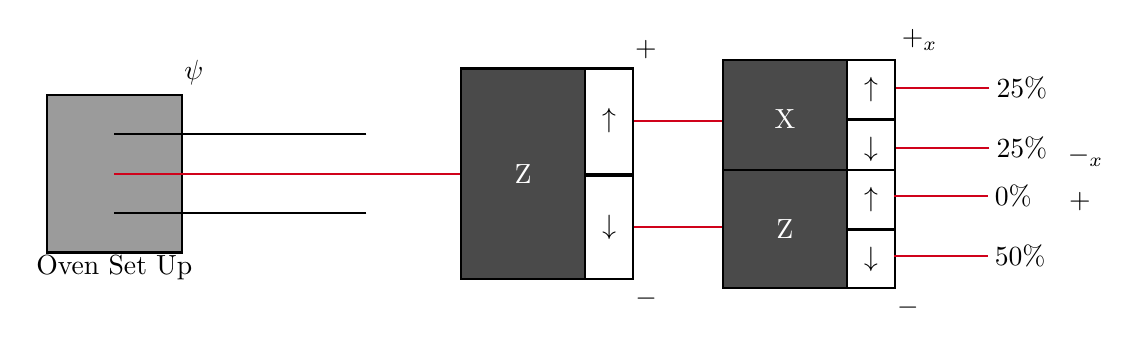
\begin{tikzpicture}[x=0.75pt,y=0.75pt,yscale=-1,xscale=1]
%uncomment if require: \path (0,375); %set diagram left start at 0, and has height of 375

%Shape: Rectangle [id:dp14421103605944618] 
\draw  [fill={rgb, 255:red, 155; green, 155; blue, 155 }  ,fill opacity=1 ] (13.01,128) -- (78.24,128) -- (78.24,204) -- (13.01,204) -- cycle ;
%Straight Lines [id:da6727148484422872] 
\draw [color={rgb, 255:red, 208; green, 2; blue, 27 }  ,draw opacity=1 ]   (167.01,166) -- (45.63,166) ;
%Shape: Rectangle [id:dp31052784363324215] 
\draw  [fill={rgb, 255:red, 74; green, 74; blue, 74 }  ,fill opacity=1 ] (212.51,115.36) -- (272.59,115.36) -- (272.59,216.64) -- (212.51,216.64) -- cycle ;
%Straight Lines [id:da9714115391207371] 
\draw    (167.01,147) -- (45.63,147) ;
%Straight Lines [id:da9565511475124852] 
\draw    (167.01,185) -- (45.63,185) ;
%Straight Lines [id:da5775689584288694] 
\draw [color={rgb, 255:red, 208; green, 2; blue, 27 }  ,draw opacity=1 ]   (212.01,166) -- (167.01,166) ;
%Shape: Rectangle [id:dp34780699384586333] 
\draw  [fill={rgb, 255:red, 255; green, 255; blue, 255 }  ,fill opacity=1 ] (272.59,167) -- (295.4,167) -- (295.4,216.64) -- (272.59,216.64) -- cycle ;
%Shape: Rectangle [id:dp9674012952324293] 
\draw  [fill={rgb, 255:red, 255; green, 255; blue, 255 }  ,fill opacity=1 ] (272.59,115.36) -- (295.4,115.36) -- (295.4,166) -- (272.59,166) -- cycle ;
%Straight Lines [id:da8039050506004896] 
\draw [color={rgb, 255:red, 208; green, 2; blue, 27 }  ,draw opacity=1 ]   (341.01,140.68) -- (296.01,140.68) ;
%Straight Lines [id:da5371523365899473] 
\draw [color={rgb, 255:red, 208; green, 2; blue, 27 }  ,draw opacity=1 ]   (341.01,191.82) -- (296.01,191.82) ;
%Shape: Rectangle [id:dp5066877735662358] 
\draw  [fill={rgb, 255:red, 74; green, 74; blue, 74 }  ,fill opacity=1 ] (338.68,111.36) -- (398.77,111.36) -- (398.77,168) -- (338.68,168) -- cycle ;
%Shape: Rectangle [id:dp7068517018359358] 
\draw  [fill={rgb, 255:red, 255; green, 255; blue, 255 }  ,fill opacity=1 ] (398.77,140.24) -- (421.58,140.24) -- (421.58,168) -- (398.77,168) -- cycle ;
%Shape: Rectangle [id:dp5547396655118183] 
\draw  [fill={rgb, 255:red, 255; green, 255; blue, 255 }  ,fill opacity=1 ] (398.77,111.36) -- (421.58,111.36) -- (421.58,139.68) -- (398.77,139.68) -- cycle ;

%Straight Lines [id:da925156022518015] 
\draw [color={rgb, 255:red, 208; green, 2; blue, 27 }  ,draw opacity=1 ]   (467.19,124.68) -- (422.19,124.68) ;
%Straight Lines [id:da995628624290608] 
\draw [color={rgb, 255:red, 208; green, 2; blue, 27 }  ,draw opacity=1 ]   (467.19,153.82) -- (422.19,153.82) ;
%Shape: Rectangle [id:dp6769071252491495] 
\draw  [fill={rgb, 255:red, 74; green, 74; blue, 74 }  ,fill opacity=1 ] (338.68,164.36) -- (398.77,164.36) -- (398.77,221) -- (338.68,221) -- cycle ;
%Shape: Rectangle [id:dp6306771616992262] 
\draw  [fill={rgb, 255:red, 255; green, 255; blue, 255 }  ,fill opacity=1 ] (398.77,193.24) -- (421.58,193.24) -- (421.58,221) -- (398.77,221) -- cycle ;
%Shape: Rectangle [id:dp43240360470130335] 
\draw  [fill={rgb, 255:red, 255; green, 255; blue, 255 }  ,fill opacity=1 ] (398.77,164.36) -- (421.58,164.36) -- (421.58,192.68) -- (398.77,192.68) -- cycle ;

%Straight Lines [id:da3774129227180918] 
\draw [color={rgb, 255:red, 208; green, 2; blue, 27 }  ,draw opacity=1 ]   (466.33,176.68) -- (421.33,176.68) ;
%Straight Lines [id:da9566074019333357] 
\draw [color={rgb, 255:red, 208; green, 2; blue, 27 }  ,draw opacity=1 ]   (466.33,205.82) -- (421.33,205.82) ;

% Text Node
\draw (45.63,204) node [anchor=north] [inner sep=0.75pt]   [align=left] {\begin{minipage}[lt]{61.13pt}\setlength\topsep{0pt}
\begin{center}
Oven Set Up
\end{center}

\end{minipage}};
% Text Node
\draw (242.55,166) node  [color={rgb, 255:red, 255; green, 255; blue, 255 }  ,opacity=1 ] [align=left] {Z};
% Text Node
\draw (284,140.68) node    {$\uparrow $};
% Text Node
\draw (284,191.82) node  [rotate=-180]  {$\uparrow $};
% Text Node
\draw (77.91,124.6) node [anchor=south west] [inner sep=0.75pt]    {$\ket{\psi }$};
% Text Node
\draw (295.07,111.96) node [anchor=south west] [inner sep=0.75pt]    {$\ket{+}$};
% Text Node
\draw (295.14,220.04) node [anchor=north west][inner sep=0.75pt]    {$\ket{-}$};
% Text Node
\draw (423.58,107.96) node [anchor=south west] [inner sep=0.75pt]    {$\ket{+}_{x}$};
% Text Node
\draw (421.32,224.4) node [anchor=north west][inner sep=0.75pt]    {$\ket{-}$};
% Text Node
\draw (368.73,139.68) node  [color={rgb, 255:red, 255; green, 255; blue, 255 }  ,opacity=1 ] [align=left] {X};
% Text Node
\draw (410.17,125.52) node    {$\uparrow $};
% Text Node
\draw (410.17,154.12) node  [rotate=-180]  {$\uparrow $};
% Text Node
\draw (410.17,207.12) node  [rotate=-180]  {$\uparrow $};
% Text Node
\draw (410.17,178.52) node    {$\uparrow $};
% Text Node
\draw (368.73,192.68) node  [color={rgb, 255:red, 255; green, 255; blue, 255 }  ,opacity=1 ] [align=left] {Z};
% Text Node
\draw (468.33,176.68) node [anchor=west] [inner sep=0.75pt]    {$0\%$};
% Text Node
\draw (468.33,205.82) node [anchor=west] [inner sep=0.75pt]    {$50\%$};
% Text Node
\draw (504.2,185.28) node [anchor=south west] [inner sep=0.75pt]    {$\ket{+}$};
% Text Node
\draw (503.58,163.96) node [anchor=south west] [inner sep=0.75pt]    {$\ket{-}_{x}$};
% Text Node
\draw (469.19,124.68) node [anchor=west] [inner sep=0.75pt]    {$25\%$};
% Text Node
\draw (469.19,153.82) node [anchor=west] [inner sep=0.75pt]    {$25\%$};


\end{tikzpicture}
